\documentclass[]{article}
\usepackage{lmodern}
\usepackage{amssymb,amsmath}
\usepackage{ifxetex,ifluatex}
\usepackage{fixltx2e} % provides \textsubscript
\ifnum 0\ifxetex 1\fi\ifluatex 1\fi=0 % if pdftex
  \usepackage[T1]{fontenc}
  \usepackage[utf8]{inputenc}
\else % if luatex or xelatex
  \ifxetex
    \usepackage{mathspec}
  \else
    \usepackage{fontspec}
  \fi
  \defaultfontfeatures{Ligatures=TeX,Scale=MatchLowercase}
\fi
% use upquote if available, for straight quotes in verbatim environments
\IfFileExists{upquote.sty}{\usepackage{upquote}}{}
% use microtype if available
\IfFileExists{microtype.sty}{%
\usepackage{microtype}
\UseMicrotypeSet[protrusion]{basicmath} % disable protrusion for tt fonts
}{}
\usepackage[margin=1in]{geometry}
\usepackage{hyperref}
\hypersetup{unicode=true,
            pdftitle={From zero to bioinformatics in R},
            pdfauthor={Jonathan Dreyfuss PhD, Assoc Dir, Bioinfo \& Biostat Core, Joslin Diabetes Center},
            pdfborder={0 0 0},
            breaklinks=true}
\urlstyle{same}  % don't use monospace font for urls
\usepackage{color}
\usepackage{fancyvrb}
\newcommand{\VerbBar}{|}
\newcommand{\VERB}{\Verb[commandchars=\\\{\}]}
\DefineVerbatimEnvironment{Highlighting}{Verbatim}{commandchars=\\\{\}}
% Add ',fontsize=\small' for more characters per line
\usepackage{framed}
\definecolor{shadecolor}{RGB}{248,248,248}
\newenvironment{Shaded}{\begin{snugshade}}{\end{snugshade}}
\newcommand{\KeywordTok}[1]{\textcolor[rgb]{0.13,0.29,0.53}{\textbf{#1}}}
\newcommand{\DataTypeTok}[1]{\textcolor[rgb]{0.13,0.29,0.53}{#1}}
\newcommand{\DecValTok}[1]{\textcolor[rgb]{0.00,0.00,0.81}{#1}}
\newcommand{\BaseNTok}[1]{\textcolor[rgb]{0.00,0.00,0.81}{#1}}
\newcommand{\FloatTok}[1]{\textcolor[rgb]{0.00,0.00,0.81}{#1}}
\newcommand{\ConstantTok}[1]{\textcolor[rgb]{0.00,0.00,0.00}{#1}}
\newcommand{\CharTok}[1]{\textcolor[rgb]{0.31,0.60,0.02}{#1}}
\newcommand{\SpecialCharTok}[1]{\textcolor[rgb]{0.00,0.00,0.00}{#1}}
\newcommand{\StringTok}[1]{\textcolor[rgb]{0.31,0.60,0.02}{#1}}
\newcommand{\VerbatimStringTok}[1]{\textcolor[rgb]{0.31,0.60,0.02}{#1}}
\newcommand{\SpecialStringTok}[1]{\textcolor[rgb]{0.31,0.60,0.02}{#1}}
\newcommand{\ImportTok}[1]{#1}
\newcommand{\CommentTok}[1]{\textcolor[rgb]{0.56,0.35,0.01}{\textit{#1}}}
\newcommand{\DocumentationTok}[1]{\textcolor[rgb]{0.56,0.35,0.01}{\textbf{\textit{#1}}}}
\newcommand{\AnnotationTok}[1]{\textcolor[rgb]{0.56,0.35,0.01}{\textbf{\textit{#1}}}}
\newcommand{\CommentVarTok}[1]{\textcolor[rgb]{0.56,0.35,0.01}{\textbf{\textit{#1}}}}
\newcommand{\OtherTok}[1]{\textcolor[rgb]{0.56,0.35,0.01}{#1}}
\newcommand{\FunctionTok}[1]{\textcolor[rgb]{0.00,0.00,0.00}{#1}}
\newcommand{\VariableTok}[1]{\textcolor[rgb]{0.00,0.00,0.00}{#1}}
\newcommand{\ControlFlowTok}[1]{\textcolor[rgb]{0.13,0.29,0.53}{\textbf{#1}}}
\newcommand{\OperatorTok}[1]{\textcolor[rgb]{0.81,0.36,0.00}{\textbf{#1}}}
\newcommand{\BuiltInTok}[1]{#1}
\newcommand{\ExtensionTok}[1]{#1}
\newcommand{\PreprocessorTok}[1]{\textcolor[rgb]{0.56,0.35,0.01}{\textit{#1}}}
\newcommand{\AttributeTok}[1]{\textcolor[rgb]{0.77,0.63,0.00}{#1}}
\newcommand{\RegionMarkerTok}[1]{#1}
\newcommand{\InformationTok}[1]{\textcolor[rgb]{0.56,0.35,0.01}{\textbf{\textit{#1}}}}
\newcommand{\WarningTok}[1]{\textcolor[rgb]{0.56,0.35,0.01}{\textbf{\textit{#1}}}}
\newcommand{\AlertTok}[1]{\textcolor[rgb]{0.94,0.16,0.16}{#1}}
\newcommand{\ErrorTok}[1]{\textcolor[rgb]{0.64,0.00,0.00}{\textbf{#1}}}
\newcommand{\NormalTok}[1]{#1}
\usepackage{graphicx,grffile}
\makeatletter
\def\maxwidth{\ifdim\Gin@nat@width>\linewidth\linewidth\else\Gin@nat@width\fi}
\def\maxheight{\ifdim\Gin@nat@height>\textheight\textheight\else\Gin@nat@height\fi}
\makeatother
% Scale images if necessary, so that they will not overflow the page
% margins by default, and it is still possible to overwrite the defaults
% using explicit options in \includegraphics[width, height, ...]{}
\setkeys{Gin}{width=\maxwidth,height=\maxheight,keepaspectratio}
\IfFileExists{parskip.sty}{%
\usepackage{parskip}
}{% else
\setlength{\parindent}{0pt}
\setlength{\parskip}{6pt plus 2pt minus 1pt}
}
\setlength{\emergencystretch}{3em}  % prevent overfull lines
\providecommand{\tightlist}{%
  \setlength{\itemsep}{0pt}\setlength{\parskip}{0pt}}
\setcounter{secnumdepth}{0}
% Redefines (sub)paragraphs to behave more like sections
\ifx\paragraph\undefined\else
\let\oldparagraph\paragraph
\renewcommand{\paragraph}[1]{\oldparagraph{#1}\mbox{}}
\fi
\ifx\subparagraph\undefined\else
\let\oldsubparagraph\subparagraph
\renewcommand{\subparagraph}[1]{\oldsubparagraph{#1}\mbox{}}
\fi

%%% Use protect on footnotes to avoid problems with footnotes in titles
\let\rmarkdownfootnote\footnote%
\def\footnote{\protect\rmarkdownfootnote}

%%% Change title format to be more compact
\usepackage{titling}

% Create subtitle command for use in maketitle
\newcommand{\subtitle}[1]{
  \posttitle{
    \begin{center}\large#1\end{center}
    }
}

\setlength{\droptitle}{-2em}

  \title{From zero to bioinformatics in R}
    \pretitle{\vspace{\droptitle}\centering\huge}
  \posttitle{\par}
    \author{Jonathan Dreyfuss PhD, Assoc Dir, Bioinfo \& Biostat Core, Joslin
Diabetes Center}
    \preauthor{\centering\large\emph}
  \postauthor{\par}
      \predate{\centering\large\emph}
  \postdate{\par}
    \date{2019-01-15}


\begin{document}
\maketitle

\section{Welcome}\label{welcome}

You'd like to analyze and visualize your data on a computer. Your
workflow will be the most flexible, powerful, and reproducible if it
involves \emph{programming}. This type of programming is now called
\emph{data science}, and it's a hot field. In 2018, \emph{data
scientist} was the best job in America for the third year in a row
according to
\href{https://www.glassdoor.com/List/Best-Jobs-in-America-LST_KQ0,20.htm}{Glassdoor}.

Once you decide to program, you need to decide which software to use, so
(of course) we'll look at some data. Data scientist job postings on
\href{https://www.indeed.com}{Indeed} often include the free languages
\href{https://www.r-project.org/}{R} and
\href{https://www.python.org/}{Python}.

\begin{figure}
\centering
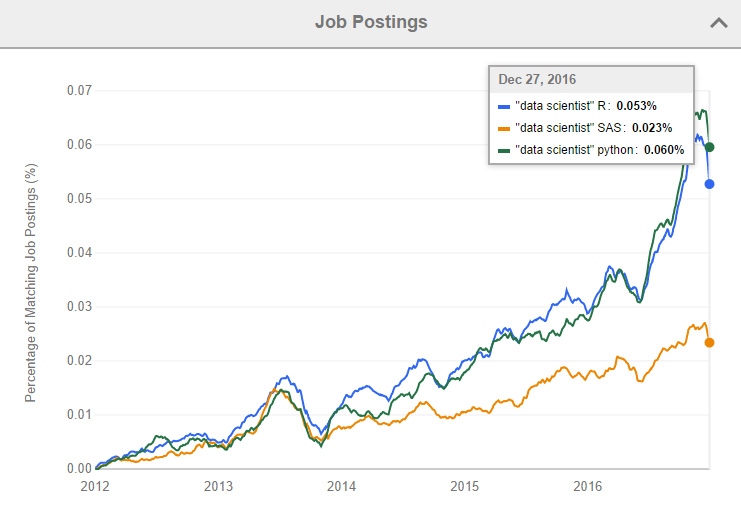
\includegraphics{job_trends.png}
\caption{\href{https://blog.revolutionanalytics.com/2017/02/job-trends-for-r-and-python.html}{Indeed
``data scientist'' job listings}}
\end{figure}

In academia, statistical software in Google Scholar papers shows that in
2016 R was the 2nd most used software and is growing. (If you're
switching from SAS or SPSS, the author of this analysis also wrote
\href{http://r4stats.com/books/r4sas-spss/}{R for SAS and SPSS Users}.)

\begin{figure}
\centering
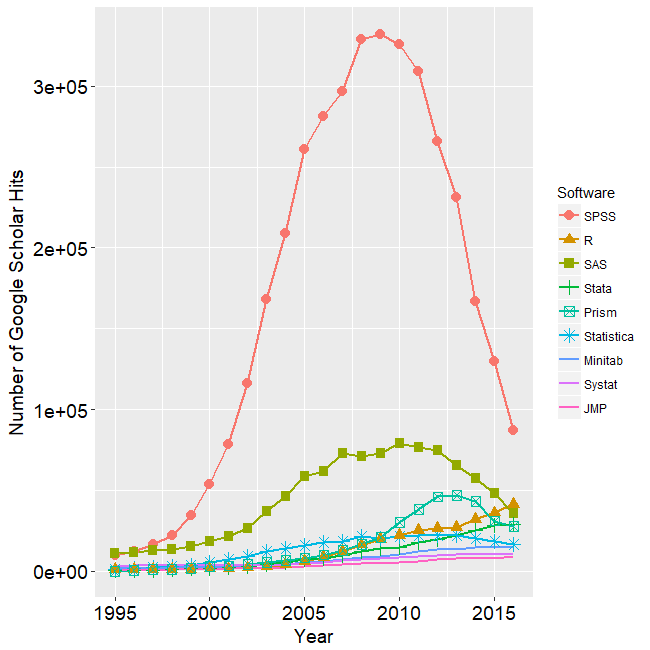
\includegraphics{Fig_2d_ScholarlyImpact2016.png}
\caption{\href{http://r4stats.com/articles/popularity/}{The Popularity
of Data Science Software, Fig 2d}}
\end{figure}

Programming looks intimidating, but once you understand the basics, you
should be able to Google questions, understand the answers, and be
productive. I'll try to teach as much of the basics as I can in the hour
I have to present this tutorial. You may wish to come back to it later
to refresh and practice.

\section{R}\label{r}

\begin{itemize}
\tightlist
\item
  R is a free language and software for statistical computing and
  graphics\\
\item
  R has thousands of free contributed packages, such as roughly 1000
  bioinformatics packages that make up the
  \href{https://www.bioconductor.org/}{Bioconductor} project, and
  packages that allow R to create data-rich, interactive
  \href{https://shiny.rstudio.com/gallery/}{websites}\\
\item
  You can download base R for
  \href{https://cloud.r-project.org/bin/windows/base/}{Windows} or
  \href{https://cloud.r-project.org/bin/macosx/}{Mac OS X} or Linux
\end{itemize}

\subsection{Resources}\label{resources}

In RStudio go to Help/R Help, then

\begin{itemize}
\tightlist
\item
  \href{https://www.rstudio.com/online-learning/}{Learning R Online}.
  One resource they cite is the free book
  \href{https://r4ds.had.co.nz/}{R for Data Science}, which has a
  particularly helpful chapter on
  \href{https://r4ds.had.co.nz/data-visualisation.html}{data
  visualization} using the popular R package \texttt{ggplot2}.\\
\item
  \emph{An Introduction to R}. The intro is also available in
  \href{http://cran.r-project.org/doc/manuals/R-intro.pdf}{PDF}. I found
  it (especially the first six chapters, which is only 30 pages) very
  helpful when I was learning R.\\
\item
  RStudio also maintains many
  \href{https://www.rstudio.com/resources/cheatsheets/}{cheatsheets},
  including for Base R
\end{itemize}

Harvard R/bioinformatics
\href{http://bioinformatics.sph.harvard.edu/training/}{trainings}

\subsection{R packages developed by the
Core}\label{r-packages-developed-by-the-core}

Dr.~Hui Pan (Bioinfo \& Biostat Core) and I have developed several R
packages to streamline bioinformatics analysis. These are based on the
popular R package
\href{https://www.ncbi.nlm.nih.gov/pmc/articles/PMC4402510/}{limma},
which applies linear modeling of omics data with sophisticated variance
estimation to improve power, and has been validated multiple times. Our
packages are freely available on the popular code repository
\href{https://github.com/}{Github}. R packages on Github can be directly
installed in R.

Our analysis package is
\href{https://github.com/jdreyf/ezlimma}{ezlimma} and our plotting
package is \href{https://github.com/jdreyf/ezlimmaplot}{ezlimmaplot},
whose README includes installation instructions for both.

\section{RStudio}\label{rstudio}

\begin{itemize}
\tightlist
\item
  \href{https://www.rstudio.com/}{RStudio} is the most popular
  integrated development environment (IDE) for R\\
\item
  We will be using R through RStudio\\
\item
  You can download
  \href{https://www.rstudio.com/products/rstudio/download/}{RStudio
  Desktop: Open Source Licence} for free
\item
  RStudio has a lot of functionality, so it will take some time to
  become comfortable with
\end{itemize}

\subsection{R Markdown}\label{r-markdown}

This report is written in \href{https://rmarkdown.rstudio.com/}{R
Markdown}, which weaves together text, figures, and code. You can
``Knit'' R Markdown documents into HTML, PDF, Microsoft Word, or other
formats by pressing the ``Knit'' icon in R Studio.

\begin{figure}
\centering
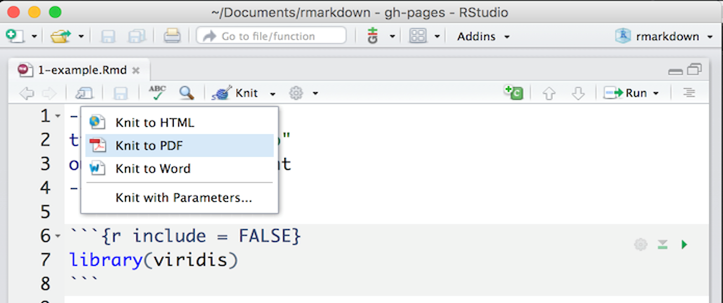
\includegraphics{knit.png}
\caption{Image from
\href{https://rmarkdown.rstudio.com/lesson-9.html}{RStudio R Markdown
lesson}}
\end{figure}

\subsection{RStudio panels}\label{rstudio-panels}

The R Markdown is in the \emph{Source} panel. This is where you write \&
save your code. The \emph{Console} is below; it executes R code. We'll
look at the other panels soon.

Press ctrl+enter (or cmd+enter on a mac) to send a line or highlighted
portion to console. When a line is executed, its return value is
displayed unless that value is assigned to a variable.

\begin{Shaded}
\begin{Highlighting}[]
\DecValTok{1}\OperatorTok{+}\DecValTok{1}
\end{Highlighting}
\end{Shaded}

\begin{verbatim}
## [1] 2
\end{verbatim}

\begin{Shaded}
\begin{Highlighting}[]
\CommentTok{# is a comment. it doesn't get executed.}
\NormalTok{x <-}\StringTok{ }\DecValTok{1}\OperatorTok{+}\DecValTok{1} \CommentTok{#nothing is displayed}
\end{Highlighting}
\end{Shaded}

\section{Types}\label{types}

\subsection{Numeric}\label{numeric}

\begin{Shaded}
\begin{Highlighting}[]
\NormalTok{x <-}\StringTok{ }\DecValTok{4} \CommentTok{#assigns the value 4 to variable x. '<-' represents an arrow.}
\NormalTok{x =}\StringTok{ }\DecValTok{4} \CommentTok{#does the same thing.  '<-' is usually equivalent to '='.}
\KeywordTok{print}\NormalTok{(x) }\CommentTok{#you can also see the value in the Environment tab in the upper right}
\end{Highlighting}
\end{Shaded}

\begin{verbatim}
## [1] 4
\end{verbatim}

\begin{Shaded}
\begin{Highlighting}[]
\NormalTok{x }\CommentTok{#same as print() when not in loop or function}
\end{Highlighting}
\end{Shaded}

\begin{verbatim}
## [1] 4
\end{verbatim}

\begin{Shaded}
\begin{Highlighting}[]
\NormalTok{x}\OperatorTok{+}\DecValTok{2}
\end{Highlighting}
\end{Shaded}

\begin{verbatim}
## [1] 6
\end{verbatim}

\begin{Shaded}
\begin{Highlighting}[]
\KeywordTok{sum}\NormalTok{(x, }\DecValTok{2}\NormalTok{) }\CommentTok{#same as x+2}
\end{Highlighting}
\end{Shaded}

\begin{verbatim}
## [1] 6
\end{verbatim}

However, R is case sensitive, so this produces an error

\begin{Shaded}
\begin{Highlighting}[]
\NormalTok{X}\OperatorTok{+}\DecValTok{2} \CommentTok{#Error: object 'X' not found}
\end{Highlighting}
\end{Shaded}

\subsection{Logicals}\label{logicals}

A logical can have the values \texttt{TRUE}, \texttt{FALSE}, and
\texttt{NA} (``Not Available''). You might see \texttt{TRUE} and
\texttt{FALSE} abbreviated as \texttt{T} and \texttt{F}, respectively,
but I don't recommend using the abbreviation. You can create logicals
with: \texttt{\textless{}}, \texttt{\textless{}=},
\texttt{\textgreater{}}, \texttt{\textgreater{}=}, \texttt{==} for
equality, \texttt{!=} for inequality. Logical operators are: \texttt{!}
for \emph{not}; \texttt{\&} for \emph{and}; \texttt{\textbar{}} for
\emph{or}.

\begin{Shaded}
\begin{Highlighting}[]
\DecValTok{4}\OperatorTok{==}\DecValTok{4} \CommentTok{#is 4 equal to 4? }
\end{Highlighting}
\end{Shaded}

\begin{verbatim}
## [1] TRUE
\end{verbatim}

\begin{Shaded}
\begin{Highlighting}[]
\DecValTok{4}\OperatorTok{!=}\DecValTok{5} \CommentTok{#is 4 not equal to 5?}
\end{Highlighting}
\end{Shaded}

\begin{verbatim}
## [1] TRUE
\end{verbatim}

\begin{Shaded}
\begin{Highlighting}[]
\NormalTok{x <-}\StringTok{ }\DecValTok{4} \OperatorTok{>}\StringTok{ }\DecValTok{5} \CommentTok{#assign the value of 4>5 (i.e. FALSE) to x}
\OperatorTok{!}\NormalTok{x }\CommentTok{#not x}
\end{Highlighting}
\end{Shaded}

\begin{verbatim}
## [1] TRUE
\end{verbatim}

\begin{Shaded}
\begin{Highlighting}[]
\NormalTok{x }\OperatorTok{|}\StringTok{ }\NormalTok{(}\DecValTok{5}\OperatorTok{>}\DecValTok{4}\NormalTok{)}
\end{Highlighting}
\end{Shaded}

\begin{verbatim}
## [1] TRUE
\end{verbatim}

\begin{Shaded}
\begin{Highlighting}[]
\NormalTok{x }\OperatorTok{&}\StringTok{ }\OtherTok{TRUE}
\end{Highlighting}
\end{Shaded}

\begin{verbatim}
## [1] FALSE
\end{verbatim}

An easy mistake is to check equality with \texttt{=}.

\begin{Shaded}
\begin{Highlighting}[]
\DecValTok{4}\NormalTok{=}\DecValTok{4} \CommentTok{#doesn't work, '=' is for assigning values to variables}
\end{Highlighting}
\end{Shaded}

We use logicals in \texttt{if} statements.

\begin{Shaded}
\begin{Highlighting}[]
\NormalTok{z <-}\StringTok{ }\DecValTok{3}
\ControlFlowTok{if}\NormalTok{ (z}\OperatorTok{==}\DecValTok{3}\NormalTok{)\{ }
  \KeywordTok{print}\NormalTok{(}\StringTok{'z is 3'}\NormalTok{) }
\NormalTok{\}}
\end{Highlighting}
\end{Shaded}

\begin{verbatim}
## [1] "z is 3"
\end{verbatim}

We can also add an action if our condition is \texttt{FALSE}.

\begin{Shaded}
\begin{Highlighting}[]
\ControlFlowTok{if}\NormalTok{ (z}\OperatorTok{==}\DecValTok{4}\NormalTok{)\{ }
  \KeywordTok{print}\NormalTok{(}\StringTok{'z is 4'}\NormalTok{) }
\NormalTok{\} }\ControlFlowTok{else}\NormalTok{ \{}
  \KeywordTok{print}\NormalTok{(}\StringTok{'z is not 4'}\NormalTok{)}
\NormalTok{\}}
\end{Highlighting}
\end{Shaded}

\begin{verbatim}
## [1] "z is not 4"
\end{verbatim}

\subsection{Characters}\label{characters}

\begin{Shaded}
\begin{Highlighting}[]
\NormalTok{x <-}\StringTok{ 'hello'} \CommentTok{#a character string}
\NormalTok{x <-}\StringTok{ "hello"} \CommentTok{#same as above, can use single or double quotes}
\NormalTok{x}
\end{Highlighting}
\end{Shaded}

\begin{verbatim}
## [1] "hello"
\end{verbatim}

Can paste character strings together

\begin{Shaded}
\begin{Highlighting}[]
\KeywordTok{paste}\NormalTok{(x, }\StringTok{'world'}\NormalTok{)}
\end{Highlighting}
\end{Shaded}

\begin{verbatim}
## [1] "hello world"
\end{verbatim}

\subsection{\texorpdfstring{\texttt{NA} (\emph{Not Available})
values}{NA (Not Available) values}}\label{na-not-available-values}

This is for missing data. \texttt{NA}s are treated specially.

\begin{Shaded}
\begin{Highlighting}[]
\NormalTok{y <-}\StringTok{ }\OtherTok{NA} \CommentTok{#data for y is missing}
\NormalTok{y}\OperatorTok{+}\DecValTok{1} \CommentTok{#don't know y, so the result is also missing}
\end{Highlighting}
\end{Shaded}

\begin{verbatim}
## [1] NA
\end{verbatim}

\begin{Shaded}
\begin{Highlighting}[]
\KeywordTok{is.na}\NormalTok{(y) }\CommentTok{#test if a value is NA}
\end{Highlighting}
\end{Shaded}

\begin{verbatim}
## [1] TRUE
\end{verbatim}

\begin{Shaded}
\begin{Highlighting}[]
\KeywordTok{sum}\NormalTok{(y, }\DecValTok{1}\NormalTok{, }\DataTypeTok{na.rm=}\OtherTok{TRUE}\NormalTok{) }\CommentTok{#ignore NAs in sum}
\end{Highlighting}
\end{Shaded}

\begin{verbatim}
## [1] 1
\end{verbatim}

\subsection{Getting help}\label{getting-help}

To get help on \texttt{sum()} function, can Google: ``r sum'' or ``sum
in r''. If you know the function name, you can search R Studio's
\emph{Help} tab in the bottom right panel with:

\begin{Shaded}
\begin{Highlighting}[]
\NormalTok{?sum}
\end{Highlighting}
\end{Shaded}

\subsection{\texorpdfstring{Change types, called
\emph{coercion}}{Change types, called coercion}}\label{change-types-called-coercion}

Functions sometimes need input to be of a particular type, e.g.~can
coerce numbers to character.

\begin{Shaded}
\begin{Highlighting}[]
\KeywordTok{as.character}\NormalTok{(z) }\CommentTok{#can tell it's a character because it's now in quotes}
\end{Highlighting}
\end{Shaded}

\begin{verbatim}
## [1] "3"
\end{verbatim}

\begin{Shaded}
\begin{Highlighting}[]
\CommentTok{#or logical to numeric}
\KeywordTok{as.numeric}\NormalTok{(}\OtherTok{TRUE}\NormalTok{) }\CommentTok{#1}
\end{Highlighting}
\end{Shaded}

\begin{verbatim}
## [1] 1
\end{verbatim}

\begin{Shaded}
\begin{Highlighting}[]
\KeywordTok{as.numeric}\NormalTok{(}\OtherTok{FALSE}\NormalTok{) }\CommentTok{#0}
\end{Highlighting}
\end{Shaded}

\begin{verbatim}
## [1] 0
\end{verbatim}

\section{Vectors}\label{vectors}

We want a variable to be able to hold more than a single value. A vector
is a list of values of a common type (e.g.~numbers). We can do similar
operations as above to multiple values in a vector simultaneously.

\subsection{Numeric vectors}\label{numeric-vectors}

\begin{Shaded}
\begin{Highlighting}[]
\NormalTok{x <-}\StringTok{ }\KeywordTok{c}\NormalTok{(}\DecValTok{1}\NormalTok{, }\DecValTok{2}\NormalTok{, }\DecValTok{3}\NormalTok{, }\DecValTok{4}\NormalTok{) }\CommentTok{#c() is concatenation -- it creates a vector}
\NormalTok{x}
\end{Highlighting}
\end{Shaded}

\begin{verbatim}
## [1] 1 2 3 4
\end{verbatim}

We can also use \texttt{:} to create a continuous sequence

\begin{Shaded}
\begin{Highlighting}[]
\NormalTok{x <-}\StringTok{ }\DecValTok{1}\OperatorTok{:}\DecValTok{4}
\NormalTok{x}
\end{Highlighting}
\end{Shaded}

\begin{verbatim}
## [1] 1 2 3 4
\end{verbatim}

\subsubsection{Practice using functions}\label{practice-using-functions}

A more general way than \texttt{:} to create sequences is \texttt{seq()}
function. Can learn about this with

\begin{Shaded}
\begin{Highlighting}[]
\NormalTok{?seq}
\end{Highlighting}
\end{Shaded}

The following calls are the same

\begin{Shaded}
\begin{Highlighting}[]
\KeywordTok{seq}\NormalTok{(}\DecValTok{1}\NormalTok{,}\DecValTok{4}\NormalTok{,}\DecValTok{1}\NormalTok{)}
\end{Highlighting}
\end{Shaded}

\begin{verbatim}
## [1] 1 2 3 4
\end{verbatim}

\begin{Shaded}
\begin{Highlighting}[]
\CommentTok{#R expects arguments in the given order, but you can name them & give in any order}
\KeywordTok{seq}\NormalTok{(}\DataTypeTok{to=}\DecValTok{4}\NormalTok{, }\DataTypeTok{from=}\DecValTok{1}\NormalTok{, }\DataTypeTok{by=}\DecValTok{1}\NormalTok{)}
\end{Highlighting}
\end{Shaded}

\begin{verbatim}
## [1] 1 2 3 4
\end{verbatim}

\begin{Shaded}
\begin{Highlighting}[]
\CommentTok{#You don't always need to write out full argument names}
\CommentTok{#it matches "fr" to argument "from", since no other arguments start w/ "fr"}
\KeywordTok{seq}\NormalTok{(}\DataTypeTok{to=}\DecValTok{4}\NormalTok{, }\DataTypeTok{fr=}\DecValTok{1}\NormalTok{, }\DataTypeTok{by=}\DecValTok{1}\NormalTok{)}
\end{Highlighting}
\end{Shaded}

\begin{verbatim}
## [1] 1 2 3 4
\end{verbatim}

\begin{Shaded}
\begin{Highlighting}[]
\CommentTok{#You don't need to specify arguments that already have the proper default}
\KeywordTok{seq}\NormalTok{(}\DataTypeTok{to=}\DecValTok{4}\NormalTok{, }\DataTypeTok{by=}\DecValTok{1}\NormalTok{) }\CommentTok{#since default for from=1}
\end{Highlighting}
\end{Shaded}

\begin{verbatim}
## [1] 1 2 3 4
\end{verbatim}

\subsubsection{Operations on numeric
vectors}\label{operations-on-numeric-vectors}

\begin{Shaded}
\begin{Highlighting}[]
\NormalTok{y <-}\StringTok{ }\DecValTok{2}\OperatorTok{*}\NormalTok{x}\OperatorTok{+}\DecValTok{1} \CommentTok{#operates on each element of x}
\NormalTok{y}
\end{Highlighting}
\end{Shaded}

\begin{verbatim}
## [1] 3 5 7 9
\end{verbatim}

\begin{Shaded}
\begin{Highlighting}[]
\KeywordTok{mean}\NormalTok{(x)}
\end{Highlighting}
\end{Shaded}

\begin{verbatim}
## [1] 2.5
\end{verbatim}

\begin{Shaded}
\begin{Highlighting}[]
\KeywordTok{length}\NormalTok{(x) }\CommentTok{#length of vector}
\end{Highlighting}
\end{Shaded}

\begin{verbatim}
## [1] 4
\end{verbatim}

\begin{Shaded}
\begin{Highlighting}[]
\KeywordTok{var}\NormalTok{(x) }\CommentTok{#variance}
\end{Highlighting}
\end{Shaded}

\begin{verbatim}
## [1] 1.666667
\end{verbatim}

\begin{Shaded}
\begin{Highlighting}[]
\KeywordTok{t.test}\NormalTok{(x, y)}
\end{Highlighting}
\end{Shaded}

\begin{verbatim}
## 
##  Welch Two Sample t-test
## 
## data:  x and y
## t = -2.4249, df = 4.4118, p-value = 0.06646
## alternative hypothesis: true difference in means is not equal to 0
## 95 percent confidence interval:
##  -7.3641672  0.3641672
## sample estimates:
## mean of x mean of y 
##       2.5       6.0
\end{verbatim}

\begin{Shaded}
\begin{Highlighting}[]
\CommentTok{#we can repeat values using rep()}
\KeywordTok{rep}\NormalTok{(x, }\DataTypeTok{times=}\DecValTok{2}\NormalTok{)}
\end{Highlighting}
\end{Shaded}

\begin{verbatim}
## [1] 1 2 3 4 1 2 3 4
\end{verbatim}

\begin{Shaded}
\begin{Highlighting}[]
\KeywordTok{rep}\NormalTok{(x, }\DataTypeTok{each=}\DecValTok{2}\NormalTok{)}
\end{Highlighting}
\end{Shaded}

\begin{verbatim}
## [1] 1 1 2 2 3 3 4 4
\end{verbatim}

\subsection{Logical vectors}\label{logical-vectors}

\begin{Shaded}
\begin{Highlighting}[]
\NormalTok{b1 <-}\StringTok{ }\NormalTok{y }\OperatorTok{>}\StringTok{ }\DecValTok{6} \CommentTok{#is each element of y greater than 6?}
\NormalTok{b1}
\end{Highlighting}
\end{Shaded}

\begin{verbatim}
## [1] FALSE FALSE  TRUE  TRUE
\end{verbatim}

\begin{Shaded}
\begin{Highlighting}[]
\NormalTok{b2 <-}\StringTok{ }\NormalTok{y }\OperatorTok{==}\StringTok{ }\DecValTok{7} \CommentTok{#is each element of y equal to 7?}
\NormalTok{b1 }\OperatorTok{&}\StringTok{ }\NormalTok{b2 }\CommentTok{#and}
\end{Highlighting}
\end{Shaded}

\begin{verbatim}
## [1] FALSE FALSE  TRUE FALSE
\end{verbatim}

\begin{Shaded}
\begin{Highlighting}[]
\NormalTok{b1 }\OperatorTok{|}\StringTok{ }\NormalTok{b2 }\CommentTok{#or}
\end{Highlighting}
\end{Shaded}

\begin{verbatim}
## [1] FALSE FALSE  TRUE  TRUE
\end{verbatim}

\begin{Shaded}
\begin{Highlighting}[]
\OperatorTok{!}\NormalTok{b1 }\CommentTok{#not}
\end{Highlighting}
\end{Shaded}

\begin{verbatim}
## [1]  TRUE  TRUE FALSE FALSE
\end{verbatim}

\begin{Shaded}
\begin{Highlighting}[]
\CommentTok{#which values are TRUE?}
\KeywordTok{which}\NormalTok{(b1)}
\end{Highlighting}
\end{Shaded}

\begin{verbatim}
## [1] 3 4
\end{verbatim}

\begin{Shaded}
\begin{Highlighting}[]
\CommentTok{#some functions automatically coerce logicals to numeric}
\KeywordTok{sum}\NormalTok{(b1)}
\end{Highlighting}
\end{Shaded}

\begin{verbatim}
## [1] 2
\end{verbatim}

\begin{Shaded}
\begin{Highlighting}[]
\KeywordTok{mean}\NormalTok{(b1)}
\end{Highlighting}
\end{Shaded}

\begin{verbatim}
## [1] 0.5
\end{verbatim}

\subsection{Character vectors}\label{character-vectors}

\begin{Shaded}
\begin{Highlighting}[]
\NormalTok{first.names <-}\StringTok{ }\KeywordTok{c}\NormalTok{(}\StringTok{'Frederick'}\NormalTok{, }\StringTok{'Charles'}\NormalTok{)}
\NormalTok{last.names <-}\StringTok{ }\KeywordTok{c}\NormalTok{(}\StringTok{'Banting'}\NormalTok{, }\StringTok{'Best'}\NormalTok{)}
\CommentTok{#combine first & last names to make full names}
\KeywordTok{paste}\NormalTok{(first.names, last.names)}
\end{Highlighting}
\end{Shaded}

\begin{verbatim}
## [1] "Frederick Banting" "Charles Best"
\end{verbatim}

\subsection{Names}\label{names}

Elements of vectors can have names. We can create a vector with names
using the concatenation function \texttt{c()}.

\begin{Shaded}
\begin{Highlighting}[]
\NormalTok{x <-}\StringTok{ }\KeywordTok{c}\NormalTok{(}\DataTypeTok{a=}\DecValTok{4}\NormalTok{, }\DataTypeTok{b=}\DecValTok{5}\NormalTok{, }\DataTypeTok{c=}\DecValTok{6}\NormalTok{)}
\NormalTok{x}
\end{Highlighting}
\end{Shaded}

\begin{verbatim}
## a b c 
## 4 5 6
\end{verbatim}

\begin{Shaded}
\begin{Highlighting}[]
\KeywordTok{names}\NormalTok{(x) }\CommentTok{#this is itself a vector}
\end{Highlighting}
\end{Shaded}

\begin{verbatim}
## [1] "a" "b" "c"
\end{verbatim}

\subsection{Subset vectors}\label{subset-vectors}

We can subset with square brackets using indices or names.

\begin{Shaded}
\begin{Highlighting}[]
\CommentTok{#select 1st element}
\NormalTok{x[}\DecValTok{1}\NormalTok{]}
\end{Highlighting}
\end{Shaded}

\begin{verbatim}
## a 
## 4
\end{verbatim}

\begin{Shaded}
\begin{Highlighting}[]
\NormalTok{x[}\StringTok{"a"}\NormalTok{]}
\end{Highlighting}
\end{Shaded}

\begin{verbatim}
## a 
## 4
\end{verbatim}

\begin{Shaded}
\begin{Highlighting}[]
\CommentTok{#can select 2nd & 3rd element in multiple ways}
\NormalTok{x[}\DecValTok{2}\OperatorTok{:}\DecValTok{3}\NormalTok{]}
\end{Highlighting}
\end{Shaded}

\begin{verbatim}
## b c 
## 5 6
\end{verbatim}

\begin{Shaded}
\begin{Highlighting}[]
\NormalTok{x[}\KeywordTok{c}\NormalTok{(}\DecValTok{2}\NormalTok{,}\DecValTok{3}\NormalTok{)]}
\end{Highlighting}
\end{Shaded}

\begin{verbatim}
## b c 
## 5 6
\end{verbatim}

\begin{Shaded}
\begin{Highlighting}[]
\NormalTok{x[}\KeywordTok{c}\NormalTok{(}\StringTok{"b"}\NormalTok{, }\StringTok{"c"}\NormalTok{)]}
\end{Highlighting}
\end{Shaded}

\begin{verbatim}
## b c 
## 5 6
\end{verbatim}

\begin{Shaded}
\begin{Highlighting}[]
\NormalTok{x[}\KeywordTok{c}\NormalTok{(}\OtherTok{FALSE}\NormalTok{, }\OtherTok{TRUE}\NormalTok{, }\OtherTok{TRUE}\NormalTok{)]}
\end{Highlighting}
\end{Shaded}

\begin{verbatim}
## b c 
## 5 6
\end{verbatim}

\begin{Shaded}
\begin{Highlighting}[]
\NormalTok{x[}\OperatorTok{-}\DecValTok{1}\NormalTok{] }\CommentTok{#all elements except the 1st}
\end{Highlighting}
\end{Shaded}

\begin{verbatim}
## b c 
## 5 6
\end{verbatim}

\section{Matrices \& Data frames}\label{matrices-data-frames}

Matrix is a table of elements of a common type.

\begin{Shaded}
\begin{Highlighting}[]
\NormalTok{m <-}\StringTok{ }\KeywordTok{matrix}\NormalTok{(}\DecValTok{1}\OperatorTok{:}\DecValTok{4}\NormalTok{, }\DataTypeTok{ncol=}\DecValTok{2}\NormalTok{, }\DataTypeTok{nrow=}\DecValTok{2}\NormalTok{) }\CommentTok{#create a numeric matrix}
\NormalTok{m }\CommentTok{#can also double-click on "m" in upper right panel, Environment tab}
\end{Highlighting}
\end{Shaded}

\begin{verbatim}
##      [,1] [,2]
## [1,]    1    3
## [2,]    2    4
\end{verbatim}

\begin{Shaded}
\begin{Highlighting}[]
\DecValTok{2}\OperatorTok{*}\NormalTok{m}\OperatorTok{+}\DecValTok{1} \CommentTok{#operates on each element}
\end{Highlighting}
\end{Shaded}

\begin{verbatim}
##      [,1] [,2]
## [1,]    3    7
## [2,]    5    9
\end{verbatim}

\begin{Shaded}
\begin{Highlighting}[]
\NormalTok{m <-}\StringTok{ }\KeywordTok{matrix}\NormalTok{(}\KeywordTok{c}\NormalTok{(}\StringTok{'a'}\NormalTok{, }\StringTok{'b'}\NormalTok{, }\StringTok{'c'}\NormalTok{, }\StringTok{'d'}\NormalTok{), }\DataTypeTok{ncol=}\DecValTok{2}\NormalTok{, }\DataTypeTok{nrow=}\DecValTok{2}\NormalTok{) }\CommentTok{#create a character matrix}
\CommentTok{#can also create by column-binding using cbind() or row-binding using rbind()}
\NormalTok{m <-}\StringTok{ }\KeywordTok{cbind}\NormalTok{(first.names, last.names)}
\end{Highlighting}
\end{Shaded}

\subsection{Matrices can have rownames \&
colnames}\label{matrices-can-have-rownames-colnames}

\begin{Shaded}
\begin{Highlighting}[]
\KeywordTok{colnames}\NormalTok{(m)}
\end{Highlighting}
\end{Shaded}

\begin{verbatim}
## [1] "first.names" "last.names"
\end{verbatim}

\begin{Shaded}
\begin{Highlighting}[]
\KeywordTok{rownames}\NormalTok{(m)}
\end{Highlighting}
\end{Shaded}

\begin{verbatim}
## NULL
\end{verbatim}

\begin{Shaded}
\begin{Highlighting}[]
\KeywordTok{rownames}\NormalTok{(m) <-}\StringTok{ }\KeywordTok{c}\NormalTok{(}\StringTok{"FB"}\NormalTok{, }\StringTok{"CB"}\NormalTok{)}
\NormalTok{m}
\end{Highlighting}
\end{Shaded}

\begin{verbatim}
##    first.names last.names
## FB "Frederick" "Banting" 
## CB "Charles"   "Best"
\end{verbatim}

We can subset matrices \& data frames using
\texttt{object{[}rows,\ columns{]}}. As with vectors, we can specify
these using indices or names.

\begin{Shaded}
\begin{Highlighting}[]
\NormalTok{m[}\DecValTok{1}\NormalTok{,] }\CommentTok{#1st row; leaving the columns index empty selects all columns}
\end{Highlighting}
\end{Shaded}

\begin{verbatim}
## first.names  last.names 
## "Frederick"   "Banting"
\end{verbatim}

\begin{Shaded}
\begin{Highlighting}[]
\NormalTok{m[,}\DecValTok{1}\NormalTok{] }\CommentTok{#1st column}
\end{Highlighting}
\end{Shaded}

\begin{verbatim}
##          FB          CB 
## "Frederick"   "Charles"
\end{verbatim}

\begin{Shaded}
\begin{Highlighting}[]
\NormalTok{m[}\StringTok{'FB'}\NormalTok{,] }\CommentTok{#1st row}
\end{Highlighting}
\end{Shaded}

\begin{verbatim}
## first.names  last.names 
## "Frederick"   "Banting"
\end{verbatim}

\begin{Shaded}
\begin{Highlighting}[]
\NormalTok{m[}\DecValTok{2}\NormalTok{,}\DecValTok{1}\NormalTok{] }\CommentTok{#2nd row, 1st column}
\end{Highlighting}
\end{Shaded}

\begin{verbatim}
## [1] "Charles"
\end{verbatim}

\begin{Shaded}
\begin{Highlighting}[]
\NormalTok{m[,}\StringTok{'first.names'}\NormalTok{] }\CommentTok{#1st column}
\end{Highlighting}
\end{Shaded}

\begin{verbatim}
##          FB          CB 
## "Frederick"   "Charles"
\end{verbatim}

\subsection{Data frames}\label{data-frames}

A data frame is a table where columns can be of different types but
elements within a column are of a common type, like a vector. This is
the type of table you'll likely use most of the time.

\subsubsection{\texorpdfstring{\texttt{data.frame}}{data.frame}}\label{data.frame}

Can create data frame using \texttt{data.frame}

\begin{Shaded}
\begin{Highlighting}[]
\NormalTok{d <-}\StringTok{ }\KeywordTok{data.frame}\NormalTok{(first.names, last.names, }\DataTypeTok{num=}\DecValTok{1}\OperatorTok{:}\DecValTok{2}\NormalTok{)}
\KeywordTok{colnames}\NormalTok{(d)}
\end{Highlighting}
\end{Shaded}

\begin{verbatim}
## [1] "first.names" "last.names"  "num"
\end{verbatim}

\begin{Shaded}
\begin{Highlighting}[]
\KeywordTok{rownames}\NormalTok{(d) <-}\StringTok{ }\KeywordTok{c}\NormalTok{(}\StringTok{"FB"}\NormalTok{, }\StringTok{"CB"}\NormalTok{)}
\NormalTok{d[}\KeywordTok{c}\NormalTok{(}\StringTok{"FB"}\NormalTok{, }\StringTok{"CB"}\NormalTok{), }\DecValTok{2}\NormalTok{]}
\end{Highlighting}
\end{Shaded}

\begin{verbatim}
## [1] Banting Best   
## Levels: Banting Best
\end{verbatim}

\begin{Shaded}
\begin{Highlighting}[]
\NormalTok{d[,}\KeywordTok{c}\NormalTok{(}\StringTok{'first.names'}\NormalTok{, }\StringTok{'num'}\NormalTok{)]}
\end{Highlighting}
\end{Shaded}

\begin{verbatim}
##    first.names num
## FB   Frederick   1
## CB     Charles   2
\end{verbatim}

\begin{Shaded}
\begin{Highlighting}[]
\CommentTok{#can also use $ for data frame columns}
\NormalTok{d}\OperatorTok{$}\NormalTok{first.names}
\end{Highlighting}
\end{Shaded}

\begin{verbatim}
## [1] Frederick Charles  
## Levels: Charles Frederick
\end{verbatim}

\section{Object info}\label{object-info}

Can get detailed info about objects with \texttt{summary()} or
\texttt{str()}

\begin{Shaded}
\begin{Highlighting}[]
\KeywordTok{summary}\NormalTok{(d)}
\end{Highlighting}
\end{Shaded}

\begin{verbatim}
##     first.names   last.names      num      
##  Charles  :1    Banting:1    Min.   :1.00  
##  Frederick:1    Best   :1    1st Qu.:1.25  
##                              Median :1.50  
##                              Mean   :1.50  
##                              3rd Qu.:1.75  
##                              Max.   :2.00
\end{verbatim}

\begin{Shaded}
\begin{Highlighting}[]
\KeywordTok{str}\NormalTok{(d) }\CommentTok{#shows structure}
\end{Highlighting}
\end{Shaded}

\begin{verbatim}
## 'data.frame':    2 obs. of  3 variables:
##  $ first.names: Factor w/ 2 levels "Charles","Frederick": 2 1
##  $ last.names : Factor w/ 2 levels "Banting","Best": 1 2
##  $ num        : int  1 2
\end{verbatim}

\section{Factors}\label{factors}

Notice that the columns are factors. R turns characters into factors
when reading/making tables by default. Factors are a special data type
with levels. Factors can be difficult to use, so avoid when possible.

\begin{Shaded}
\begin{Highlighting}[]
\CommentTok{#we can coerce factors to character}
\NormalTok{d[,}\DecValTok{1}\NormalTok{] <-}\StringTok{ }\KeywordTok{as.character}\NormalTok{(d[,}\DecValTok{1}\NormalTok{])}
\KeywordTok{str}\NormalTok{(d) }\CommentTok{#1st column is now character}
\end{Highlighting}
\end{Shaded}

\begin{verbatim}
## 'data.frame':    2 obs. of  3 variables:
##  $ first.names: chr  "Frederick" "Charles"
##  $ last.names : Factor w/ 2 levels "Banting","Best": 1 2
##  $ num        : int  1 2
\end{verbatim}

We can also prevent R from turning characters into factors by setting a
global option

\begin{Shaded}
\begin{Highlighting}[]
\KeywordTok{options}\NormalTok{(}\DataTypeTok{stringsAsFactors=}\OtherTok{FALSE}\NormalTok{) }\CommentTok{#applies to the rest of your session}
\NormalTok{d2 <-}\StringTok{ }\KeywordTok{data.frame}\NormalTok{(first.names, last.names, }\DataTypeTok{num=}\DecValTok{1}\OperatorTok{:}\DecValTok{2}\NormalTok{)}
\KeywordTok{str}\NormalTok{(d2) }\CommentTok{#no factors}
\end{Highlighting}
\end{Shaded}

\begin{verbatim}
## 'data.frame':    2 obs. of  3 variables:
##  $ first.names: chr  "Frederick" "Charles"
##  $ last.names : chr  "Banting" "Best"
##  $ num        : int  1 2
\end{verbatim}

\section{Lists}\label{lists}

Lists are arbitrary collections of objects. The elements don't have to
form a rectangular table or be of a common type. Lists can also be
difficult to use, but you probably won't use them directly much.

\begin{Shaded}
\begin{Highlighting}[]
\NormalTok{l <-}\StringTok{ }\KeywordTok{list}\NormalTok{(}\DataTypeTok{pathway1=}\KeywordTok{c}\NormalTok{(}\StringTok{'gene1'}\NormalTok{, }\StringTok{'gene2'}\NormalTok{), }\DataTypeTok{pathway2=}\KeywordTok{c}\NormalTok{(}\StringTok{'gene3'}\NormalTok{, }\StringTok{'gene4'}\NormalTok{, }\StringTok{'gene5'}\NormalTok{))}
\NormalTok{l}
\end{Highlighting}
\end{Shaded}

\begin{verbatim}
## $pathway1
## [1] "gene1" "gene2"
## 
## $pathway2
## [1] "gene3" "gene4" "gene5"
\end{verbatim}

We can select using names with \texttt{\$}, like columns of a data frame
(a data frame is actually a list under the hood).

\begin{Shaded}
\begin{Highlighting}[]
\NormalTok{l}\OperatorTok{$}\NormalTok{pathway1}
\end{Highlighting}
\end{Shaded}

\begin{verbatim}
## [1] "gene1" "gene2"
\end{verbatim}

Some functions return lists. For example, rownames and colnames of a
matrix are together called dimnames, which is a list of length 2.

\begin{Shaded}
\begin{Highlighting}[]
\KeywordTok{dimnames}\NormalTok{(m)}
\end{Highlighting}
\end{Shaded}

\begin{verbatim}
## [[1]]
## [1] "FB" "CB"
## 
## [[2]]
## [1] "first.names" "last.names"
\end{verbatim}

\begin{Shaded}
\begin{Highlighting}[]
\KeywordTok{length}\NormalTok{(}\KeywordTok{dimnames}\NormalTok{(m))}
\end{Highlighting}
\end{Shaded}

\begin{verbatim}
## [1] 2
\end{verbatim}

Another function that returns a list is correlation with
\texttt{cor.test()}.

\begin{Shaded}
\begin{Highlighting}[]
\NormalTok{?cor.test }\CommentTok{#in documentation, "Value" section says it returns a list}
\end{Highlighting}
\end{Shaded}

\begin{Shaded}
\begin{Highlighting}[]
\NormalTok{ct <-}\StringTok{ }\KeywordTok{cor.test}\NormalTok{(}\DecValTok{1}\OperatorTok{:}\DecValTok{3}\NormalTok{, }\KeywordTok{c}\NormalTok{(}\DecValTok{6}\NormalTok{,}\DecValTok{5}\NormalTok{,}\DecValTok{7}\NormalTok{))}
\NormalTok{ct}\OperatorTok{$}\NormalTok{p.value}
\end{Highlighting}
\end{Shaded}

\begin{verbatim}
## [1] 0.6666667
\end{verbatim}

\section{Example data set}\label{example-data-set}

We'll work with a simulated gene expression matrix, such as from a
microarray, with 100 genes \& 9 samples, split into 3 groups.
\texttt{rnorm()} randomly simulates normally distributed values. We make
the 1st gene up-regulated in group `a'.

We're going to treat this data as being already \emph{processed}. For
many datasets, there are zeroes or missing values that might need to be
imputed; samples need to be normalized to make them comparable and
amenable to statistical tests; absent genes need to be removed; sample
outliers need to be assessed to examine whether some experimental
variables or batch effects need to be accounted for or the samples need
to be removed or down-weighted; and trends between a gene's mean
expression and its variance should be accounted for, especially in
RNA-seq data
\href{https://genomebiology.biomedcentral.com/articles/10.1186/gb-2014-15-2-r29}{voom}.

\begin{Shaded}
\begin{Highlighting}[]
\KeywordTok{set.seed}\NormalTok{(}\DecValTok{0}\NormalTok{) }\CommentTok{#set a seed for random sampling to get reproducible results}
\NormalTok{gx <-}\StringTok{ }\KeywordTok{matrix}\NormalTok{(}\KeywordTok{rnorm}\NormalTok{(}\DataTypeTok{n=}\DecValTok{900}\NormalTok{), }\DataTypeTok{nrow=}\DecValTok{100}\NormalTok{, }\DataTypeTok{ncol=}\DecValTok{9}\NormalTok{)}
\CommentTok{#sep='' says not to put a space between 'gene' and the numbers}
\NormalTok{gx[}\DecValTok{1}\NormalTok{, }\DecValTok{1}\OperatorTok{:}\DecValTok{3}\NormalTok{] <-}\StringTok{ }\NormalTok{gx[}\DecValTok{1}\NormalTok{, }\DecValTok{1}\OperatorTok{:}\DecValTok{3}\NormalTok{]}\OperatorTok{+}\DecValTok{3}
\KeywordTok{rownames}\NormalTok{(gx) <-}\StringTok{ }\KeywordTok{paste}\NormalTok{(}\StringTok{'gene'}\NormalTok{, }\DecValTok{1}\OperatorTok{:}\DecValTok{100}\NormalTok{, }\DataTypeTok{sep=}\StringTok{''}\NormalTok{)}
\CommentTok{#3 samples in group 'a' & 3 in group 'b' & 3 in group 'c'}
\KeywordTok{colnames}\NormalTok{(gx) <-}\StringTok{ }\KeywordTok{c}\NormalTok{(}\KeywordTok{paste}\NormalTok{(}\StringTok{'a'}\NormalTok{, }\DecValTok{1}\OperatorTok{:}\DecValTok{3}\NormalTok{, }\DataTypeTok{sep=}\StringTok{''}\NormalTok{), }\KeywordTok{paste}\NormalTok{(}\StringTok{'b'}\NormalTok{, }\DecValTok{1}\OperatorTok{:}\DecValTok{3}\NormalTok{, }\DataTypeTok{sep=}\StringTok{''}\NormalTok{), }\KeywordTok{paste}\NormalTok{(}\StringTok{'c'}\NormalTok{, }\DecValTok{1}\OperatorTok{:}\DecValTok{3}\NormalTok{, }\DataTypeTok{sep=}\StringTok{''}\NormalTok{))}
\end{Highlighting}
\end{Shaded}

We create matching phenotype \& annotation data frames.

\begin{Shaded}
\begin{Highlighting}[]
\NormalTok{pheno <-}\StringTok{ }\KeywordTok{data.frame}\NormalTok{(}\DataTypeTok{grp=}\KeywordTok{rep}\NormalTok{(}\KeywordTok{c}\NormalTok{(}\StringTok{'a'}\NormalTok{, }\StringTok{'b'}\NormalTok{, }\StringTok{'c'}\NormalTok{), }\DataTypeTok{each=}\DecValTok{3}\NormalTok{))}
\KeywordTok{rownames}\NormalTok{(pheno) <-}\StringTok{ }\KeywordTok{colnames}\NormalTok{(gx)}

\CommentTok{# make random gene symbols: don't worry about how i generate these}
\NormalTok{annot <-}\StringTok{ }\KeywordTok{data.frame}\NormalTok{(}\DataTypeTok{gene.symbols=}\KeywordTok{paste0}\NormalTok{(}\KeywordTok{sample}\NormalTok{(}\DataTypeTok{x=}\NormalTok{LETTERS, }\DataTypeTok{size=}\DecValTok{100}\NormalTok{, }\DataTypeTok{replace=}\OtherTok{TRUE}\NormalTok{), }
                                        \KeywordTok{sample}\NormalTok{(}\DataTypeTok{x=}\NormalTok{LETTERS, }\DataTypeTok{size=}\DecValTok{100}\NormalTok{, }\DataTypeTok{replace=}\OtherTok{TRUE}\NormalTok{), }
                                        \KeywordTok{sample}\NormalTok{(}\DataTypeTok{x=}\NormalTok{LETTERS, }\DataTypeTok{size=}\DecValTok{100}\NormalTok{, }\DataTypeTok{replace=}\OtherTok{TRUE}\NormalTok{)))}
\KeywordTok{rownames}\NormalTok{(annot) <-}\StringTok{ }\KeywordTok{rownames}\NormalTok{(gx)}
\end{Highlighting}
\end{Shaded}

\section{Reading / writing data}\label{reading-writing-data}

We're going to write \& read from the working directory. R assumes by
default that you're reading/writing in your working directory.

\begin{Shaded}
\begin{Highlighting}[]
\KeywordTok{getwd}\NormalTok{() }\CommentTok{#see working directory}
\end{Highlighting}
\end{Shaded}

\begin{verbatim}
## [1] "B:/fcns/zero2bioinfo"
\end{verbatim}

We can change working directory with \texttt{setwd()} or under
Session/Set Working Directory. Usually we write to tab-delimited text
(TXT) or comma separated value (CSV). Both can be opened in Excel, and
Excel can save as both formats.

\begin{Shaded}
\begin{Highlighting}[]
\KeywordTok{write.csv}\NormalTok{(gx, }\StringTok{"gx.csv"}\NormalTok{) }\CommentTok{#now look in your working directory for the file}
\CommentTok{#tables are read in by default as data frames}
\NormalTok{gx <-}\StringTok{ }\KeywordTok{read.csv}\NormalTok{(}\StringTok{"gx.csv"}\NormalTok{, }\DataTypeTok{row.names=}\DecValTok{1}\NormalTok{) }\CommentTok{#row.names=1 sets 1st column as rownames}
\CommentTok{#transform gx from data.frame to a numeric matrix}
\NormalTok{gx <-}\StringTok{ }\KeywordTok{data.matrix}\NormalTok{(gx)}
\end{Highlighting}
\end{Shaded}

\section{Many types of plots are
available}\label{many-types-of-plots-are-available}

Can see in R Studio in bottom right \emph{Plots} tab

\begin{Shaded}
\begin{Highlighting}[]
\KeywordTok{boxplot}\NormalTok{(gx)}
\end{Highlighting}
\end{Shaded}

\includegraphics{zero2bioinfo_files/figure-latex/unnamed-chunk-38-1.pdf}

\begin{Shaded}
\begin{Highlighting}[]
\KeywordTok{hist}\NormalTok{(gx)}
\end{Highlighting}
\end{Shaded}

\includegraphics{zero2bioinfo_files/figure-latex/unnamed-chunk-38-2.pdf}

Most basic is \texttt{plot()} so we'll practice with this.

\begin{Shaded}
\begin{Highlighting}[]
\KeywordTok{plot}\NormalTok{(}\DataTypeTok{x=}\NormalTok{gx[,}\DecValTok{1}\NormalTok{], }\DataTypeTok{y=}\NormalTok{gx[,}\DecValTok{2}\NormalTok{]) }\CommentTok{#scatter plot of a1 vs a2}
\end{Highlighting}
\end{Shaded}

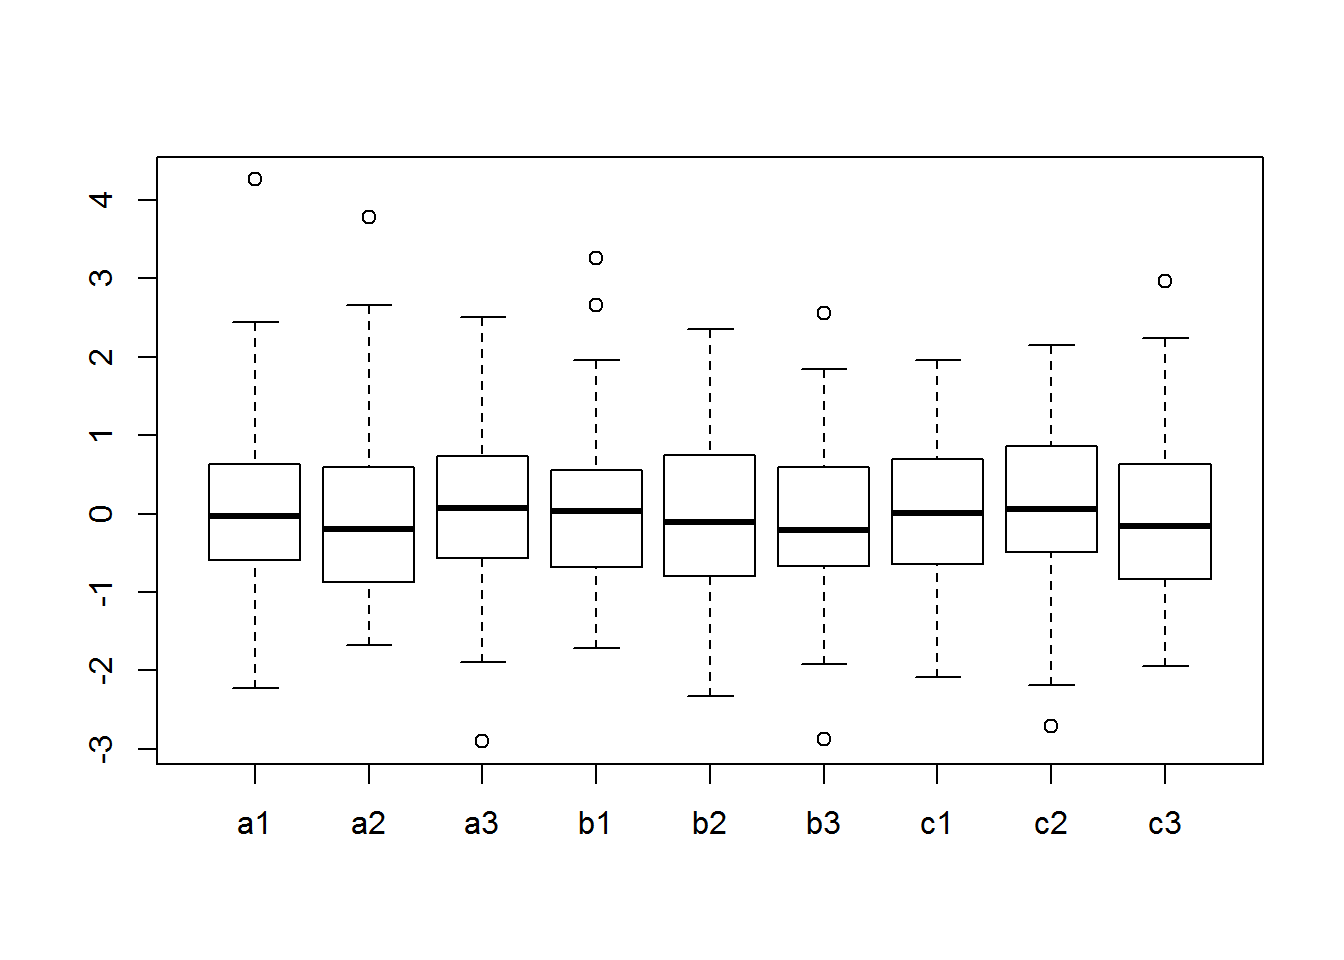
\includegraphics{zero2bioinfo_files/figure-latex/unnamed-chunk-39-1.pdf}

We want axis labels to be sample names. We find out how to do this by
looking at

\begin{Shaded}
\begin{Highlighting}[]
\NormalTok{?plot}
\end{Highlighting}
\end{Shaded}

We see that the arguments we need are:

\begin{Shaded}
\begin{Highlighting}[]
\KeywordTok{plot}\NormalTok{(}\DataTypeTok{x=}\NormalTok{gx[,}\DecValTok{1}\NormalTok{], }\DataTypeTok{y=}\NormalTok{gx[,}\DecValTok{2}\NormalTok{], }\DataTypeTok{xlab=}\KeywordTok{colnames}\NormalTok{(gx)[}\DecValTok{1}\NormalTok{], }\DataTypeTok{ylab=}\KeywordTok{colnames}\NormalTok{(gx)[}\DecValTok{2}\NormalTok{])}
\end{Highlighting}
\end{Shaded}

\includegraphics{zero2bioinfo_files/figure-latex/unnamed-chunk-41-1.pdf}

We also want to reorient axis tick labels on y-axis.

\begin{Shaded}
\begin{Highlighting}[]
\NormalTok{?plot }\CommentTok{#sends us to par. par options are applicable to many plots.}
\NormalTok{?par }\CommentTok{#there are many par options, the one we want is "las".}
\end{Highlighting}
\end{Shaded}

\begin{Shaded}
\begin{Highlighting}[]
\KeywordTok{plot}\NormalTok{(}\DataTypeTok{x=}\NormalTok{gx[,}\DecValTok{1}\NormalTok{], }\DataTypeTok{y=}\NormalTok{gx[,}\DecValTok{2}\NormalTok{], }\DataTypeTok{xlab=}\KeywordTok{colnames}\NormalTok{(gx)[}\DecValTok{1}\NormalTok{], }\DataTypeTok{ylab=}\KeywordTok{colnames}\NormalTok{(gx)[}\DecValTok{2}\NormalTok{], }\DataTypeTok{las=}\DecValTok{1}\NormalTok{)}
\end{Highlighting}
\end{Shaded}

\includegraphics{zero2bioinfo_files/figure-latex/unnamed-chunk-43-1.pdf}

\subsection{Save plot to file}\label{save-plot-to-file}

We can use ``Export'' in \emph{Plots} tab, or we can use code to open
file, plot to it, then close it. We'l make a PDF with \texttt{pdf} but
we could use \texttt{png}, \texttt{jpeg}, \texttt{tiff}, etc.

\begin{Shaded}
\begin{Highlighting}[]
\KeywordTok{pdf}\NormalTok{(}\StringTok{'scatter.pdf'}\NormalTok{) }\CommentTok{#open graphics device}
\KeywordTok{plot}\NormalTok{(}\DataTypeTok{x=}\NormalTok{gx[,}\DecValTok{1}\NormalTok{], }\DataTypeTok{y=}\NormalTok{gx[,}\DecValTok{2}\NormalTok{], }\DataTypeTok{xlab=}\KeywordTok{colnames}\NormalTok{(gx)[}\DecValTok{1}\NormalTok{], }\DataTypeTok{ylab=}\KeywordTok{colnames}\NormalTok{(gx)[}\DecValTok{2}\NormalTok{], }\DataTypeTok{las=}\DecValTok{1}\NormalTok{)}
\KeywordTok{dev.off}\NormalTok{() }\CommentTok{#close graphics device}
\end{Highlighting}
\end{Shaded}

\begin{verbatim}
## pdf 
##   2
\end{verbatim}

\section{Differential expression using base
R}\label{differential-expression-using-base-r}

\begin{enumerate}
\def\labelenumi{\arabic{enumi}.}
\tightlist
\item
  one gene at a time
\item
  \texttt{for} loop
\item
  \texttt{apply} function
\end{enumerate}

\subsection{One gene at a time.}\label{one-gene-at-a-time.}

\begin{Shaded}
\begin{Highlighting}[]
\KeywordTok{t.test}\NormalTok{(gx[}\DecValTok{1}\NormalTok{, }\DecValTok{1}\OperatorTok{:}\DecValTok{3}\NormalTok{], gx[}\DecValTok{1}\NormalTok{, }\DecValTok{4}\OperatorTok{:}\DecValTok{6}\NormalTok{])}\OperatorTok{$}\NormalTok{p.value }\CommentTok{#1st gene}
\end{Highlighting}
\end{Shaded}

\begin{verbatim}
## [1] 0.02976692
\end{verbatim}

\begin{Shaded}
\begin{Highlighting}[]
\KeywordTok{t.test}\NormalTok{(gx[}\DecValTok{2}\NormalTok{, }\DecValTok{1}\OperatorTok{:}\DecValTok{3}\NormalTok{], gx[}\DecValTok{2}\NormalTok{, }\DecValTok{4}\OperatorTok{:}\DecValTok{6}\NormalTok{])}\OperatorTok{$}\NormalTok{p.value }\CommentTok{#2nd gene}
\end{Highlighting}
\end{Shaded}

\begin{verbatim}
## [1] 0.5437477
\end{verbatim}

\subsection{\texorpdfstring{\texttt{for}
loop}{for loop}}\label{for-loop}

This can be automated using a \texttt{for} loop. We'll create a new
vector of \texttt{NA}S \& assign the t-test p-values to that vector.
This loops the variable \texttt{gene} through each of the values between
1 \& 100, and applies a t-test on that row.

\begin{Shaded}
\begin{Highlighting}[]
\NormalTok{pv <-}\StringTok{ }\KeywordTok{rep}\NormalTok{(}\OtherTok{NA}\NormalTok{, }\DataTypeTok{times=}\DecValTok{100}\NormalTok{)}
\ControlFlowTok{for}\NormalTok{ (gene }\ControlFlowTok{in} \DecValTok{1}\OperatorTok{:}\DecValTok{100}\NormalTok{)\{}
\NormalTok{  pv[gene] <-}\StringTok{ }\KeywordTok{t.test}\NormalTok{(gx[gene, }\DecValTok{1}\OperatorTok{:}\DecValTok{3}\NormalTok{], gx[gene, }\DecValTok{4}\OperatorTok{:}\DecValTok{6}\NormalTok{])}\OperatorTok{$}\NormalTok{p.value}
\NormalTok{\}}
\end{Highlighting}
\end{Shaded}

\subsection{\texorpdfstring{\texttt{apply}}{apply}}\label{apply}

There's a more advanced \& faster way you \texttt{apply} the
\texttt{t.test} function to each row.

\begin{Shaded}
\begin{Highlighting}[]
\NormalTok{pv <-}\StringTok{ }\KeywordTok{apply}\NormalTok{(gx, }\DataTypeTok{MARGIN =} \DecValTok{1}\NormalTok{, }\DataTypeTok{FUN=}\ControlFlowTok{function}\NormalTok{(row.v)\{ }
  \KeywordTok{t.test}\NormalTok{(row.v[}\DecValTok{1}\OperatorTok{:}\DecValTok{3}\NormalTok{], row.v[}\DecValTok{4}\OperatorTok{:}\DecValTok{6}\NormalTok{])}\OperatorTok{$}\NormalTok{p.value }
\NormalTok{\})}
\end{Highlighting}
\end{Shaded}

\section{\texorpdfstring{\texttt{ezlimma}
package}{ezlimma package}}\label{ezlimma-package}

You can install \texttt{ezlimma} by following instructions at
\href{https://github.com/jdreyf/ezlimma}{ezlimma}. \texttt{ezlimma}'s
tutorial is presented as a \emph{vignette}, like many R packages.

\begin{Shaded}
\begin{Highlighting}[]
\KeywordTok{library}\NormalTok{(ezlimma)}
\CommentTok{# browseVignettes(package="ezlimma")}
\end{Highlighting}
\end{Shaded}

Here we create multiple group comparisons, and test them all in one line
with \texttt{limma\_contrasts}.

\begin{Shaded}
\begin{Highlighting}[]
\NormalTok{contrast.v <-}\StringTok{ }\KeywordTok{c}\NormalTok{(}\DataTypeTok{AvsB=}\StringTok{'a-b'}\NormalTok{, }\DataTypeTok{AvsC=}\StringTok{'a-c'}\NormalTok{, }\DataTypeTok{BvsC=}\StringTok{'b-c'}\NormalTok{)}
\NormalTok{toptab <-}\StringTok{ }\KeywordTok{limma_contrasts}\NormalTok{(}\DataTypeTok{object=}\NormalTok{gx, }\DataTypeTok{grp=}\NormalTok{pheno}\OperatorTok{$}\NormalTok{grp, }\DataTypeTok{contrast.v =}\NormalTok{ contrast.v)}
\end{Highlighting}
\end{Shaded}

\texttt{toptab} is ordered by overall significance of the 3 tests. We
round the number of significant digits in \texttt{toptab} to 3 with
\texttt{signif}. When we add annotation, we make sure the rows of
\texttt{toptab} match the rows of \texttt{annot} using
\texttt{annot{[}rownames(toptab),{]}}. We write this to CSV.

\begin{Shaded}
\begin{Highlighting}[]
\NormalTok{toptab.ann <-}\StringTok{ }\KeywordTok{data.frame}\NormalTok{(}\KeywordTok{signif}\NormalTok{(toptab, }\DecValTok{3}\NormalTok{), }\DataTypeTok{symbol=}\NormalTok{annot[}\KeywordTok{rownames}\NormalTok{(toptab),])}
\KeywordTok{write.csv}\NormalTok{(toptab.ann, }\StringTok{"diff_gene_stats.csv"}\NormalTok{)}
\end{Highlighting}
\end{Shaded}

In \texttt{ezlimma}, we can also test correlation of each gene to a
continuous phenotype in one line of code.

\begin{Shaded}
\begin{Highlighting}[]
\NormalTok{Y <-}\StringTok{ }\KeywordTok{c}\NormalTok{(}\DecValTok{1}\OperatorTok{:}\DecValTok{9}\NormalTok{)}
\NormalTok{toptab.y <-}\StringTok{ }\KeywordTok{ezcor}\NormalTok{(}\DataTypeTok{object =}\NormalTok{ gx, }\DataTypeTok{phenotype =}\NormalTok{ Y, }\DataTypeTok{prefix =} \StringTok{"Y"}\NormalTok{)}
\end{Highlighting}
\end{Shaded}

\texttt{toptab.y} is ordered by the significance of the correlation and
gives correlation coefficient, p-value, and FDR.

We can plot the top gene, gene27, vs. \texttt{Y}.

\begin{Shaded}
\begin{Highlighting}[]
\KeywordTok{plot}\NormalTok{(gx[}\StringTok{"gene27"}\NormalTok{,], Y)}
\end{Highlighting}
\end{Shaded}

\includegraphics{zero2bioinfo_files/figure-latex/unnamed-chunk-52-1.pdf}

For pathway analysis, \texttt{ezlimma} extends \texttt{limma}
\texttt{roast} to write linked Excel files, as explained in the
\texttt{ezlimma} vignette.

\section{\texorpdfstring{\texttt{ezlimmaplot}
package}{ezlimmaplot package}}\label{ezlimmaplot-package}

We can plot \texttt{ezlimma} results with \texttt{ezlimmaplot}. We'll
focus on the differential expression. You can install
\texttt{ezlimmaplot} by following instructions at
\href{https://github.com/jdreyf/ezlimmaplot}{ezlimmaplot}.
\texttt{ezlimmaplot}'s tutorial is presented as a \emph{vignette}.

\begin{Shaded}
\begin{Highlighting}[]
\KeywordTok{library}\NormalTok{(ezlimmaplot)}
\CommentTok{# browseVignettes(package="ezlimmaplot")}
\end{Highlighting}
\end{Shaded}

\subsection{PCA}\label{pca}

We make a Principal Component Analysis (PCA) plot to see how samples
cluster. This is described in the \texttt{ezlimmaplot} package tutorial.

We use the \texttt{ezpca} function, which is based on the R package
\texttt{ggplot2}. We set \texttt{name=NA} so \texttt{ezpca} doesn't
print to file.

\begin{Shaded}
\begin{Highlighting}[]
\KeywordTok{ezpca}\NormalTok{(}\DataTypeTok{object=}\NormalTok{gx, }\DataTypeTok{pheno.df=}\NormalTok{pheno, }\DataTypeTok{name=}\OtherTok{NA}\NormalTok{, }\DataTypeTok{color=}\StringTok{"grp"}\NormalTok{)}
\end{Highlighting}
\end{Shaded}

\includegraphics{zero2bioinfo_files/figure-latex/unnamed-chunk-54-1.pdf}

\subsection{Significance histograms}\label{significance-histograms}

We make a histogram of p-values and false discovery rates (FDR) for each
comparison.

\begin{Shaded}
\begin{Highlighting}[]
\KeywordTok{signif_hist}\NormalTok{(}\DataTypeTok{tab =}\NormalTok{ toptab)}
\end{Highlighting}
\end{Shaded}

\subsection{Venn diagram}\label{venn-diagram}

We can see how many genes with p \textless{}= 0.05 the comparisons have
in common.

\begin{Shaded}
\begin{Highlighting}[]
\NormalTok{venn.tab <-}\StringTok{ }\KeywordTok{ezvenn}\NormalTok{(}\DataTypeTok{tab=}\NormalTok{toptab, }\DataTypeTok{name=}\OtherTok{NA}\NormalTok{, }\DataTypeTok{p.cutoff =} \FloatTok{0.05}\NormalTok{)}
\end{Highlighting}
\end{Shaded}

\includegraphics{zero2bioinfo_files/figure-latex/unnamed-chunk-56-1.pdf}

This plot doesn't tell us which genes are in common, but
\texttt{venn.tab} has this info, which we can view.

\subsection{Heatmap}\label{heatmap}

We can make a heatmap of the top genes in \texttt{toptab.ann}.

\begin{Shaded}
\begin{Highlighting}[]
\NormalTok{top.genes <-}\StringTok{ }\KeywordTok{rownames}\NormalTok{(toptab.ann)[}\DecValTok{1}\OperatorTok{:}\DecValTok{10}\NormalTok{]}
\KeywordTok{ezheat}\NormalTok{(}\DataTypeTok{object =}\NormalTok{ gx[top.genes,], }\DataTypeTok{labrows=}\NormalTok{toptab.ann[}\DecValTok{1}\OperatorTok{:}\DecValTok{10}\NormalTok{, }\StringTok{"symbol"}\NormalTok{], }\DataTypeTok{pheno.df =}\NormalTok{ pheno, }\DataTypeTok{name=}\OtherTok{NA}\NormalTok{)}
\end{Highlighting}
\end{Shaded}

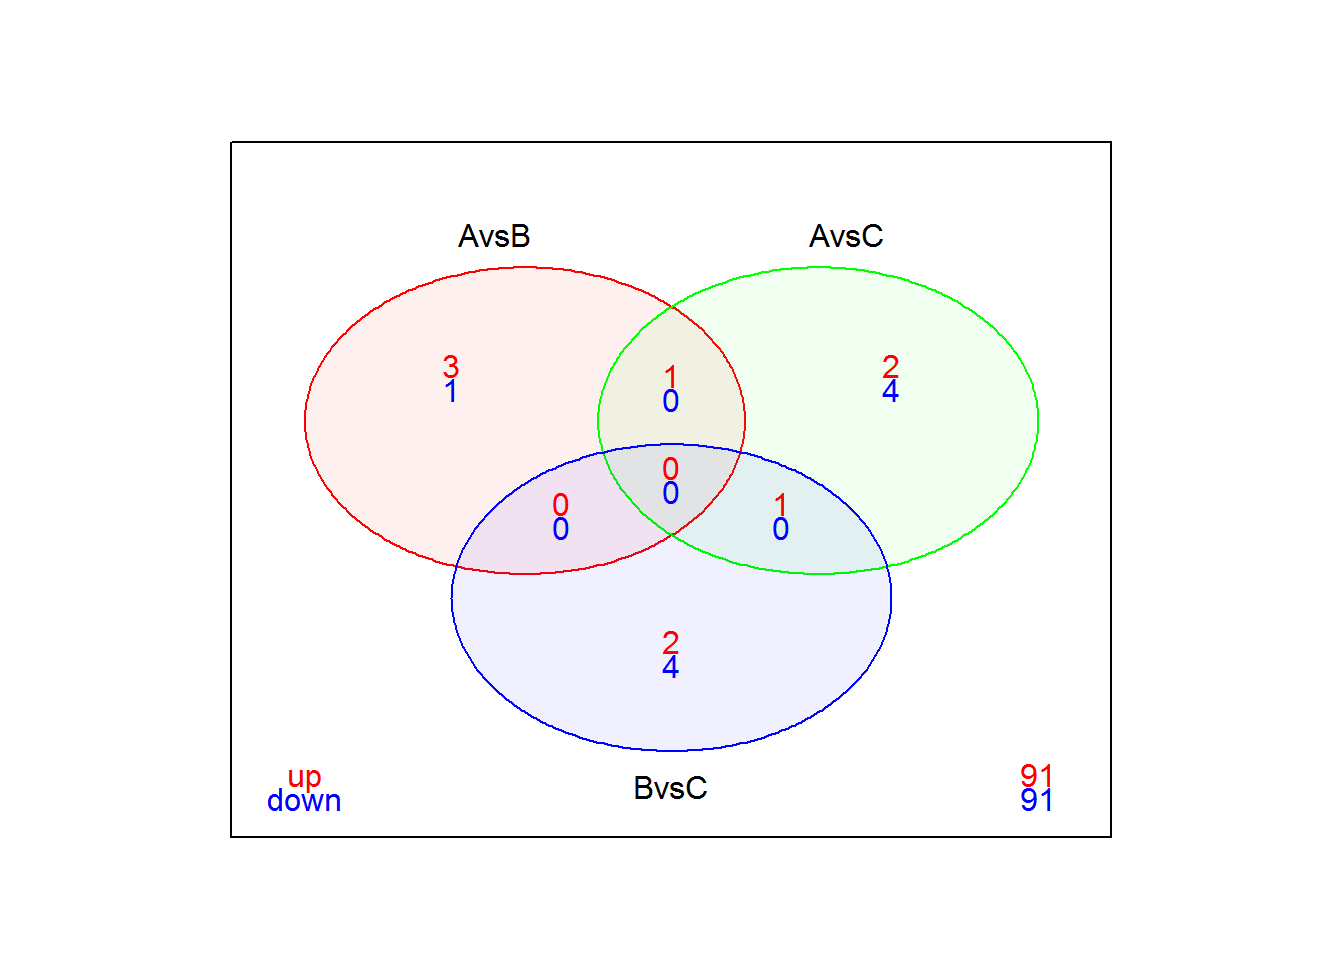
\includegraphics{zero2bioinfo_files/figure-latex/unnamed-chunk-57-1.pdf}

By default, the row scaling \emph{centers} the rows by subtracting the
row mean. Then the new mean of every row is zero. This helps see
contrast between samples, instead of between rows.

\subsection{Volcano plot}\label{volcano-plot}

We make a volcano plot for the 1st comparison, where we label the 3 most
significant genes.

\begin{Shaded}
\begin{Highlighting}[]
\KeywordTok{ezvolcano}\NormalTok{(}\DataTypeTok{tab=}\NormalTok{toptab.ann, }\DataTypeTok{ntop.sig=}\DecValTok{3}\NormalTok{, }\DataTypeTok{lab.col=}\StringTok{"symbol"}\NormalTok{, }\DataTypeTok{comparison =} \StringTok{"AvsB"}\NormalTok{, }\DataTypeTok{name=}\OtherTok{NA}\NormalTok{)}
\end{Highlighting}
\end{Shaded}

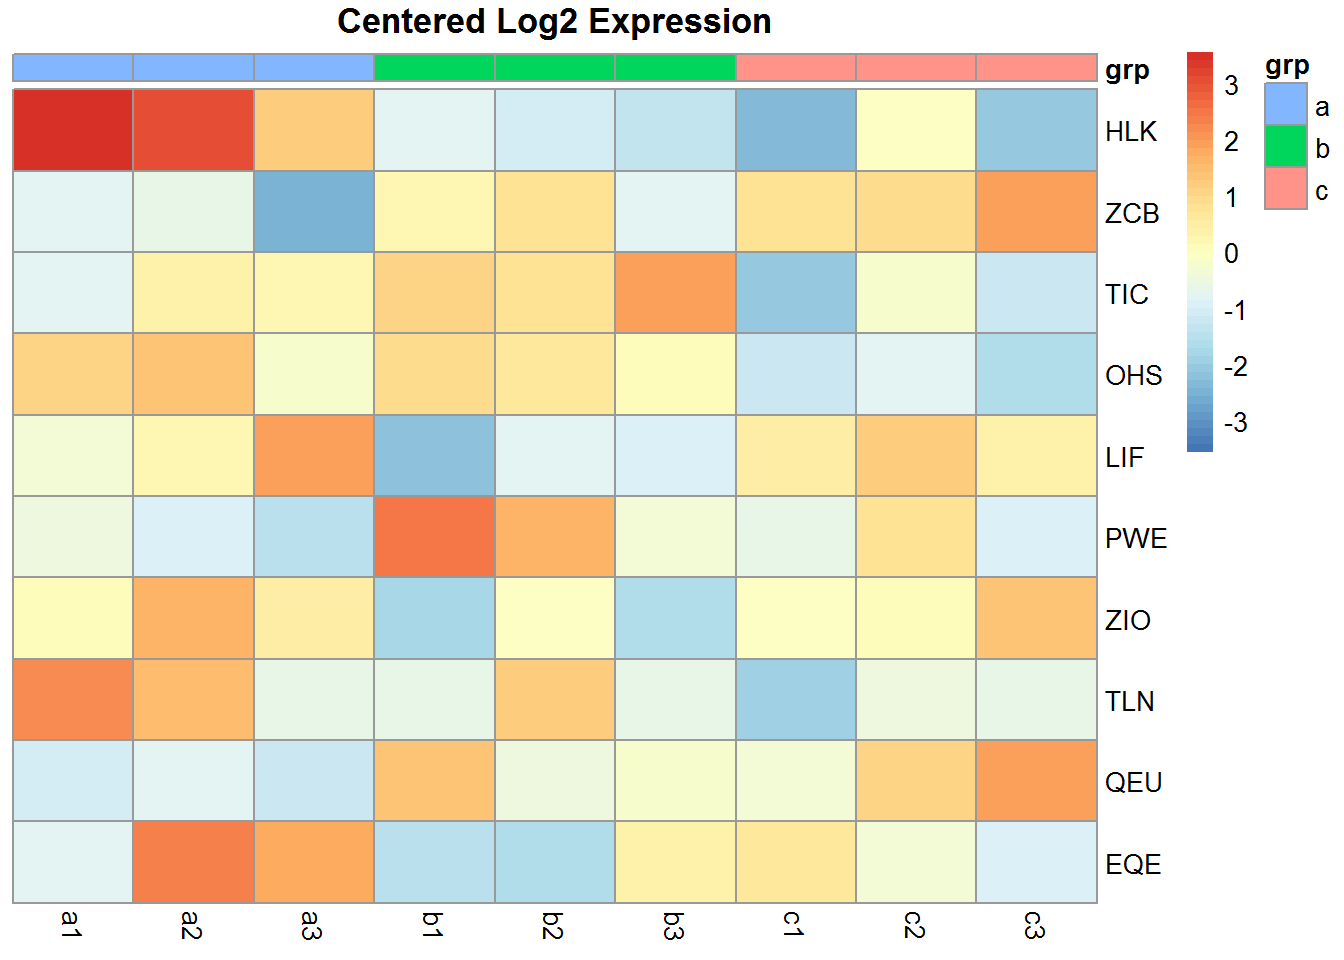
\includegraphics{zero2bioinfo_files/figure-latex/unnamed-chunk-58-1.pdf}

We can also make a volcano plot for all comparisons.

\begin{Shaded}
\begin{Highlighting}[]
\KeywordTok{multi_volcano}\NormalTok{(}\DataTypeTok{tab=}\NormalTok{toptab.ann, }\DataTypeTok{ntop.sig =} \DecValTok{3}\NormalTok{, }\DataTypeTok{lab.col=}\StringTok{"symbol"}\NormalTok{)}
\end{Highlighting}
\end{Shaded}

\section{Methods developed by the
Core}\label{methods-developed-by-the-core}

We have developed a novel method for testing causal mediation, termed
High-throughput mediation analysis (\texttt{hitman}). This is applicable
when treatment (or exposure) is randomized, and omics and an outcome
(e.g.~insulin sensitivity) are measured. Hitman then tests which
analytes best mediate the effect of the treatment on the outcome.

We have also developed a novel method for Pathway analysis via network
smoothing in the \href{https://github.com/jdreyf/PANTS}{PANTS} package.
This allows for network-based pathway mediation analysis with
\texttt{pants\_hitman}, which wasn't previously available.

These methods have been applied to test which analytes mediate the
benefit of gastric bypass on HbA1c with Dr.~ME Patti (Joslin). The paper
is currently under review. We are intrested in applying these methods
and developing new ones for new applications.

\section{Conclusion}\label{conclusion}

Congratulations for making it this far. I hope this helped you become
familiar enough with R so you can understand documentation, and
hopefully analyze your data.


\end{document}
